\documentclass[a4paper,12pt,final]{article}
\usepackage[utf8]{inputenc}
\usepackage[T1]{fontenc}
\usepackage[francais]{babel}
\usepackage{amsmath,amsfonts,amssymb}
\usepackage{graphicx}

\usepackage{fullpage}
\usepackage[amsthm]{ntheorem}
\usepackage{graphicx}

\newtheorem{Ex}{Exemple}[section]
\newtheorem{Proof}{Démonstration}[section]
\theoremstyle{theorem}
\newtheorem{Th}{Théorème}[section]
\theoremstyle{definition}
\newtheorem{Propriete}{Propriété}[section]
\theoremstyle{definition}
\newtheorem{Propos}{Proposition}[section]
\theoremstyle{definition}
\newtheorem{Def}{Définition}[section]

\linespread{1.1}


\title{CHAPITRE 2 : Expérience Aléatoire, probabilités, probabilités conditionnelles}
\author{Aurélie \textsc{Jeanmougin}}

\begin{document}
	
	\maketitle

\section{Expérience aléatoire et évènements}
	\subsection{Expérience aléatoire}
		\begin{Def}
			Une \textbf{expérience aléatoire} est une expérience renouvelable à l'identique, dont ls résultats possibles sont connus sans qu'on puisse déterminer lequel sera réalisé.
		\end{Def}
	
		\begin{Ex}
			Lancer un dé à 6 faces est une expérience renouvelable dont les résultats possibles sont tous les nombre entiers de 1 à 6.
		\end{Ex}
	
		\begin{Def}
			Les résultats possibles d'une expérience aléatoire sont appelés \textbf{éventualités} ou \textbf{issues}.
		\end{Def}
	
		\begin{Def}
			L'ensemble de toutes les issues d'une expérience aléatoire est appelé \textbf{univers}. On le note généralement $\Omega$.
		\end{Def}
		
		\begin{Ex}
			On peut reprendre l'exemple précédent : l'ensemble de toutes les issues de cette expérience aléatoire est $\Omega = \{1,2,3,4,5,6\}$.
		\end{Ex}
	
	Dans cette leçon on peut se limiter au cas où $\Omega$ est un ensemble fini.
	
	\subsection{Evénement}
		
		Un événement est associé à une expérience aléatoire, nous allons donner quelques définitions.
		
		\begin{Def}
			\begin{itemize}
				\item Un \textbf{événement} est un ensemble de plusieurs issues, c'est un sous-ensemble de $\Omega$.
				\item Un événement est dit \textbf{élémentaire} si une seule issue le réalise.
				\item L'\textbf{événement impossible} est la partie vide (noté $\emptyset$), lorsque aucune issue ne le réalise.
				\item L'\textbf{événement certain} est $\Omega$, lorsque toutes les issues le réalisent.
				\item L'\textbf{événement $A\cup B$} (lu "A union B") est constitué des issues qui appartiennent soit à A, soit à B, soit aux deux ensembles.
				\item L'\textbf{événement $A\cap B$} (lu "A inter B") est constitué des issues qui appartiennent à la fois à A et à B.
				\item Deux événements sont \textbf{incompatibles} s'ils n'ont pas l'éléments en commun, c'est-à-dire que $A\cap B = \emptyset$.
				\item L'événement $\bar{A}$ est dit \textbf{événement contraire} de A si les deux événements sont incompatibles et si l'union des deux événements forme la totalité des issues, c'est-à-dire que $A\cup \bar{A} = \Omega$ et $A\cap B = \emptyset$.
			\end{itemize}		
		\end{Def}

		\begin{Ex}
			1. Obtenir un 2 est un événement élémentaire : $\omega = \{7\}$. \\
			2. Obtenir un nombre pair est un événement : $A = \{2,4,6\}$. \\
			3. Obtenir un multiple de trois est un événement : $B = \{3,6\}$. \\
			4. $A\cap B = \{6\}$. \\
			5. $A\cup B = \{2,3,4,6\}$. \\
			6. Si on a : \[C = \{1\}\] alors $C\cap A = \emptyset$ donc C et A sont incompatibles. \\
			7. Si $\bar{A}$ est l'événement "Obtenir un nombre impair" on a : \[A\cap \bar{A} = \emptyset\]
			\[A\cup \bar{A} = \Omega\]
			
		\end{Ex}
	
		\subsection{Exercices}
			
\begin{figure}[h!]
	\centering
	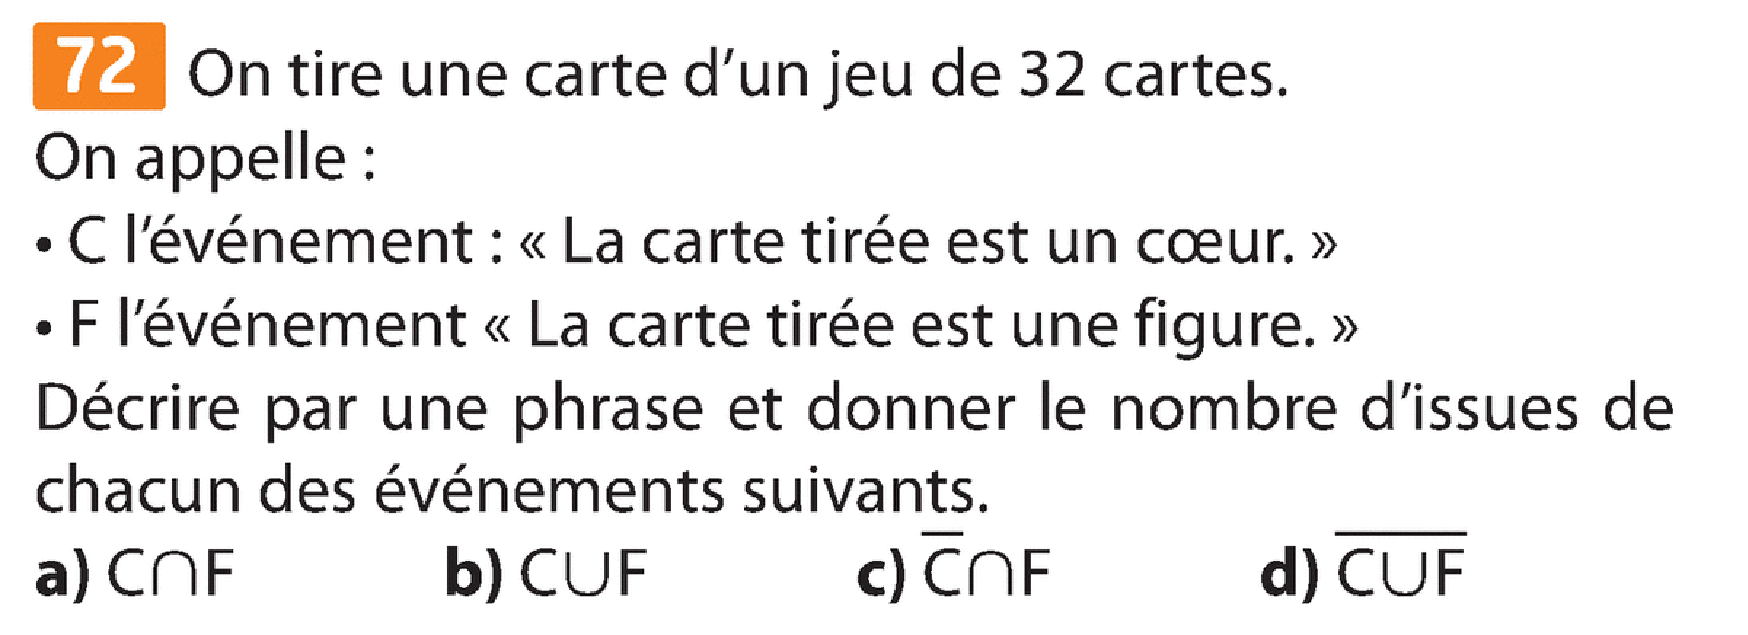
\includegraphics[width=10cm,height=5cm]{Sesamath2de_72p331.pdf}
	\caption{72 page 331 Sesamath 2nde}
	\label{fig:sesamath2de72p331}
\end{figure}
	
\section{Probabilités}
	\subsection{Arbre des possibles}
		\begin{Def}
			L'\textbf{arbre des possibles} permet de visualiser les issues d'une expérience aléatoire. On peut y noter la probabilité de chaque issue sur chacune des branches.
		\end{Def}
	
		\begin{Ex}
			Lorsque l'on fait tourner une roue de la fortune on peut modéliser chacune des issues sur un arbre des possibles.
		\end{Ex}
	\subsection{Loi de probabilités sur un univers $\Omega$}
	
		\begin{Def}
			Soit $\Omega$ l'univers d'une expérience aléatoire. On définit une loi de probabilité P sur $\Omega$ en associant à chaque événement élémentaire $\omega_{i}$ une probabilité $p_{i} \in [0,1]$ tel que :
			\[\sum_{i}p_{i} = 1\]
			On peut aussi noter $p_{i} = P(\omega_{i})$.
		\end{Def}
		
		\begin{Propos}
			La probabilité P(E) d'un événement E est la somme des probabilités des événements élémentaires qui le composent.
		\end{Propos}
	
		\begin{Ex}
			On joue avec un dé truqué. La probabilité d'apparition de chaque face est donnée ci-dessous: \[
			\begin{tabular}{|c|c|c|c|c|c|c|}
				\hline \textbf{Issue $\omega$} & 1 & 2 & 3 & 4 & 5 & 6 \\
				\hline \textbf{Probabilité $P(\omega)$} & 0,05 & 0,2 & $\alpha$ & 0,1 & 0,25 & 0,1 \\
				\hline
			\end{tabular} \]
			1. On veut calculer la probabilité de l'événement A : "Obtenir un nombre pair". D'après la définition on a :
			\[P(A) = P(2)+P(4)+P(6) = 0,2+0,1+0,1 = 0,4.\]
			2. On veut calculer la probabilité d'obtenir 3. On sait que :
			\[P(1)+P(2)+P(3)+P(4)+P(5)+P(6) = 1\]
			On a alors : 
			\[P(3) = 1 - (P(1)+P(2)+P(4)+P(5)+P(6)) = 1-(0,05+0,2+0,1+0,25+0,1) = 0,3.\]
		\end{Ex}
	
		\begin{Propriete}
			Soient A, B $\subset \Omega$. Alors :
			\begin{itemize}
				\item 1. $P(\Omega) = 1$
				\item 2. $P(\emptyset) = 0$
				\item 3. $P(\bar{A}) = 1-P(A)$
				\item 4. $P(A\setminus B) = P(A)-P(A\cap B)$
				\item 5. $A\subset B \Rightarrow P(A) \leq P(B)$
				\item 6. $P(A\cup B) = P(A)+P(B)-P(A\cap B)$
			\end{itemize}
		\end{Propriete}
	
		\begin{Proof}
			1. $P(\Omega) = P(\bigcup_{i} \omega_{i}) = \sum_{i} P(\omega_{i}) = \sum_{i}\frac{1}{n} = 1$. \\
			2. $P(A\cup \emptyset) = P(A) + P(\emptyset) \iff P(A) = P(A) + P(\emptyset)$. \\
			3. On a : $A = (A\setminus B)\cup (A\cap B)$, de plus $(A\setminus B)$ et $A\cap B$ sont disjoints donc on peut appliquer la définition : 
			\[P(A) = P(A\setminus B) + P(A\cap B)\]
			4. Comme $A\cap \bar{A} = \emptyset$ et $A\cup \bar{A} = \Omega$, on a:
			\[P(A\cup \bar{A}) = P(A) + P(\bar{A}) \iff P(\Omega) = P(A) + P(\bar{A})\]
			5. $A\subset B \Rightarrow B = (B\cap A)\cup A$ donc :
			\[P(B) = P(B\setminus A) + P(A) \leq P(A) \]
			6. On a :
			\[A\cup B = (A\setminus B)\cup (A\cap B)\cup (B\setminus A)\] 
		\end{Proof}
	
	\subsection{Equiprobabilité}
		\begin{Def}
			Si tous les éléments de $\Omega$ ont la même probabilité d'apparition alors $\Omega$ est dit \textbf{équiprobable}. Si $\Omega = \{a_{1},...,a_{n}\}$ alors : 
			\[P(\{a_{i}\}) = \frac{1}{n}, \forall a_{i} \in \Omega \] 
		\end{Def}
	
		\begin{Propriete}
			Si $\Omega$ est équiprobable, la probabilité d'un événement $A\subset \Omega$ contenant $n_{A}$ éléments est:
			\[P(A) = \frac{1}{n} + ... + \frac{1}{n} = \frac{n_{A}}{n} = \frac{card(A)}{card(\Omega)}\]
		\end{Propriete}
	
		\begin{Ex}
			On lance un dé non truqué. \\
			1. La probabilité d'obtenir 5 est : $P(5) = \frac{1}{6}$. \\
			2. La probabilité d'obtenir un nombre pair est : $P(2)+P(4)+P(6) = \frac{3}{6} = \frac{1}{2}$.
		\end{Ex}
	
	\subsection{Exercices}
		\begin{figure}[h!]
			\centering
			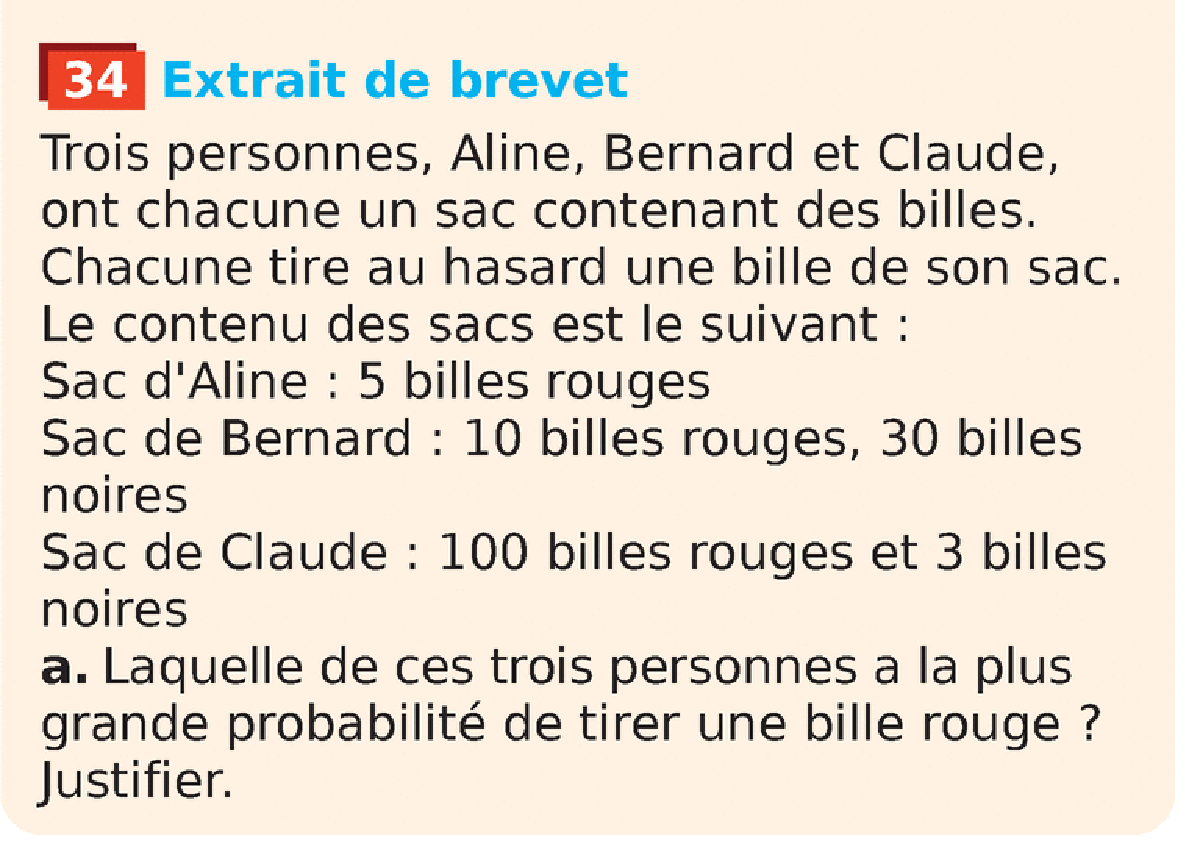
\includegraphics[width=8cm,height=8cm]{SesamathC4_34p171.pdf}
			\caption{34 page 171 Sesamath Cycle 4}
			\label{fig:sesamathc434p171}
		\end{figure}
	
		\begin{figure}[h!]
			\centering
			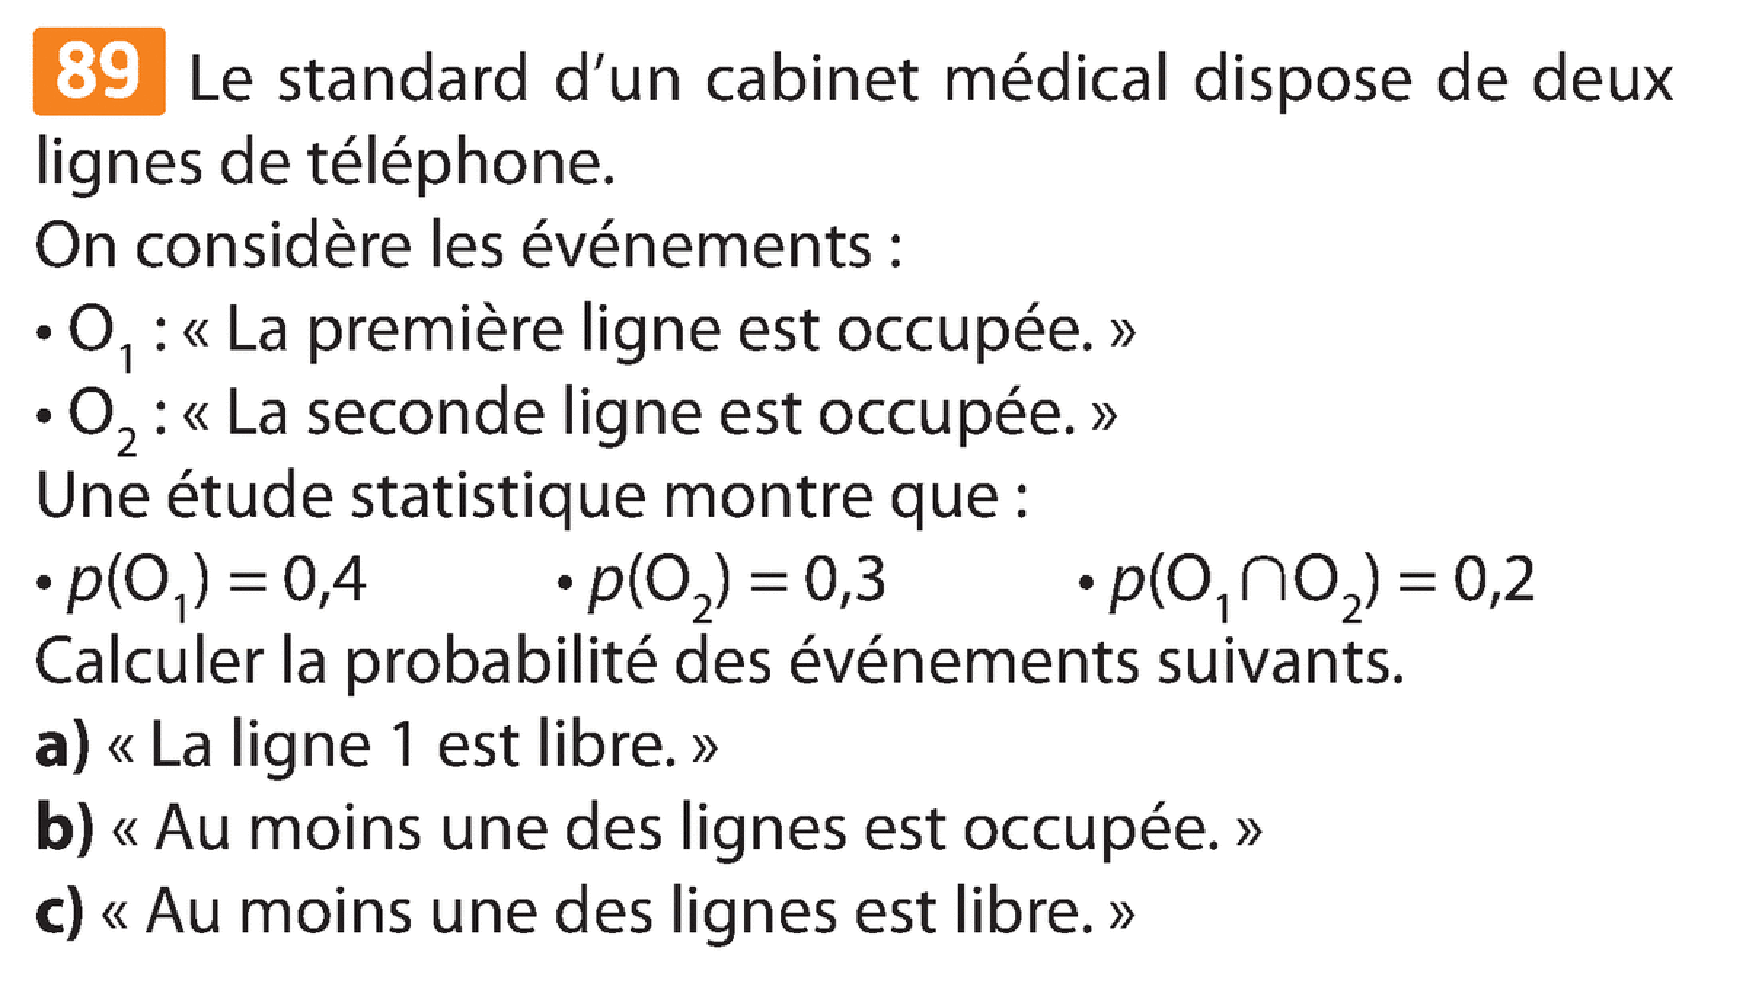
\includegraphics[width=8cm,height=7cm]{Sesamath2de_89p333.pdf}
			\caption{89 page 333 Sesamath 2nde}
			\label{fig:sesamath2de89p333}
		\end{figure}
	
\newpage	
\section{Probabilité conditionnelle}
	\subsection{Probabilité conditionnelle}
	
		\begin{Def}
			Soit A et B deux événements avec $P(A) > 0$ et $A\subset \Omega$, on appelle \textbf{probabilité conditionnelle de B sachant A}, la probabilité que l'événement B se réalise sachant que l'événement A est réalisé. Cette probabilité conditionnelle à A est l'application $P_{A}(.)$ de l'ensemble des événements ($P(\Omega)$) dans $[0,1]$ telle que :
			\[ \begin{array}{lll}
					P_{A} : &P(\Omega) &\rightarrow [0,1] \\
					&B &\mapsto P_{A}(B) = \frac{P(A\cap B)}{P(A)}
				\end{array}
			       \]
		\end{Def}
	
		\begin{Ex}
			On tire une carte au hasard dans un jeu de 32 cartes. \\
			Soit A l'événement "Le résultat est un pique". \\
			Soit B l'événement "Le résultat est un roi". \\
			Donc $A\cap B$ est l'événement "Le résultat est le roi de pique". \\
			Alors : $P(A) = \frac{8}{32} = \frac{1}{4}$ et $P(A\cap B) = \frac{1}{32}$. \\
			Donc la probabilité que le résultat soit un roi sachant qu'on a tiré une carte pique est : 
			\[P_{A}(B) = \frac{P(A\cap B)}{P(A)} = \frac{\frac{1}{32}}{\frac{1}{4}} = \frac{1}{8}\]
		\end{Ex}
	
		\begin{Propriete}
			Soit A et B deux événements avec $P(A)>0$, on a : \\
			\begin{itemize}
				\item $0 \leq P_{A}(B) \leq 1$
				\item $P_{A}(\bar{B}) = 1-P_{A}(B)$
				\item $P(A\cap B) = P_{A}(B) \times P(A) = P_{B}(A) \times P(B)$
			\end{itemize}
		\end{Propriete}
	
	\subsection{Probabilités totales et de Bayes}
		\begin{Propriete}
			\textbf{Formule des probabilités totales.} Soit $\{E_{1},...,E_{n}\}$ une partition de $\Omega$ d'événements non vides. Soit $A\subset \Omega$. Alors :
			\[P(A) = \sum_{i=1}^{n} P_{E_{i}}(A) \times P(E_{i})\]
		\end{Propriete}
		
		\begin{Ex}
			On considère deux urnes $U_{1}$ et $U_{2}$. L'urne $U_{1}$ contient 6 boules noires et 4 boules blanches. L'urne $U_{2}$ contient 3 boules noires et 7 boules blanches. On lance un dé non truqué. S'il indique le chiffre 1, on choisit l'urne $U_{1}$ sinon on choisit l'urne $U_{2}$. On effectue ensuite deux tirages avec remise. On cherche la probabilité d'avoir tiré deux boules noires en tout. On note :
			\[N = \{\text{noir au premier tirage}\}\]
			\[N' = \{\text{noir au second tirage}\}\]
			\[H_{1} = \{\text{choix de l'urne $U_{1}$}\}\]
			\[H_{2} = \bar{H_{1}} = \{\text{choix de l'urne $U_{2}$}\}\]
			On a ainsi :
			\[P_{H_{1}}(N) = \frac{6}{10} = \frac{3}{5}\]
			\[P_{H_{1}}(N\cap N') = (\frac{3}{5})^{2}\]
			\[P_{H_{2}}(N) = \frac{3}{10}\]
			\[P_{H_{2}}(N\cap N') = (\frac{3}{10})^{2}\]
			La formule nous donne alors:
			\[P(N) = P_{H_{1}}(N) \times P(H_{1}) + P_{H_{2}}(N) \times P(H_{2})\]
			\[P(N) = \frac{1}{6} \times \frac{3}{5} + \frac{5}{6} \times \frac{3}{10} = \frac{1}{10} + \frac{1}{4} = \frac{7}{20}\]
			\[P(N\cap N') = P_{H_{1}}(N\cap N') \times P(H_{1}) + P_{H_{2}}(N\cap N') \times P(H_{2})\]
			\[P(N) = \frac{1}{6} \times (\frac{3}{5})^{2} + \frac{5}{6} \times (\frac{3}{10})^{2} = \frac{27}{200}\]
			
		\end{Ex}
	
		\begin{Propriete}
			\textbf{Formule de Bayes.} Soit $\{E_{1},...,E_{n}\}$ une partition de $\Omega$ d'événements non vides. Soit $A\subset \Omega$. Alors : 
			\[P_{A}(E_{i}) = \frac{P_{E_{i}}(A) \times P(E_{i})}{\sum_{i=1}^{n}P_{E_{i}}(A) \times P(E_{i}) }\]
		\end{Propriete}
	
	\subsection{Indépendance}
		\begin{Def}
			Deux événements A et B sont \textbf{indépendants} si : \\
			\begin{itemize}
				\item $P(A\cap B) = P(A) \times P(B)$
				\item $P_{A}(B) = P(B)$
				\item $P_{B}(A) = P(A)$
			\end{itemize}
		\end{Def}
	
		\begin{Ex}
			On tire une carte au hasard dans un jeu de 32 cartes. \\
			Soit A l'événement "Le résultat est un trèfle". \\
			Soit B l'événement "Le résultat est un roi". \\
			Donc $A\cap B$ est l'événement "Le résultat est le roi de trèfle". \\
			Alors : $P(A) = \frac{8}{32} = \frac{1}{4}$, $P(B) = \frac{4}{32} = \frac{1}{8}$ et $P(A\cap B) = \frac{1}{32}$. \\
			On a donc : 
			\[P(A) \times P(B) = \frac{1}{4} \times \frac{1}{8} = \frac{1}{32} = P(A\cap B)\]
			Les événements A et B sont indépendants.
		\end{Ex}
	
		\begin{Propriete}
			Si A et B sont indépendants alors $\bar{A}$ et B sont indépendants.
		\end{Propriete}	
	
		\begin{Proof}
			\[P(\bar{A}\cap B) = P(B\cap \bar{A})\]
			\[P(\bar{A}\cap B) = P(B) \times P_{B}(\bar{A})\]
			\[P(\bar{A}\cap B) = P(B) \times (1 - P_{B}(A))\]
			\[P(\bar{A}\cap B) = P(B) \times (1 - P(A)) \text{car A et B sont indépendants}\]
			\[P(\bar{A}\cap B) = P(B) \times P(\bar{A})\]
			Donc $\bar{A}$ et B sont indépendants.
		\end{Proof}
	
	\subsection{Schéma de Bernoulli}
		\begin{Def}
			Toute expérience aléatoire conduisant à deux issues possibles S (Succès) et $\bar{S}$ (Echec) est appelée une \textbf{épreuve de Bernoulli}.
		\end{Def}
		\begin{Ex}
			Si on appelle Succès lors d'un lancé d'un dé, l'événement noté : S = "Obtenir 6". Le lancer du dé peut alors être considéré comme une épreuve de Bernoulli avec :\begin{itemize}
				\item $ S = \{6\}$ et $p = P(S) = \frac{1}{6}$.
				\item $\bar{S} = \{1,2,3,4,5\}$ et $q = 1-p = \frac{5}{6}$.
			\end{itemize}
		\end{Ex}
	
		\begin{Def}
			Si on répète $n$ fois et de façon indépendante une épreuve de Bernoulli, on obtient un \textbf{schéma de Bernoulli}.
		\end{Def}
	
		\begin{Propriete}
			Soit $0 \leq k \leq n$ avec $k,n \in \mathbb{N}$,
			\[P(\text{"Obtenir k succès"}) = \binom{n}{k}p^{k}(1-p)^{n-k}\]
		\end{Propriete}
	
	\subsection{Exercices}
		
		\begin{figure}[h!]
			\centering
			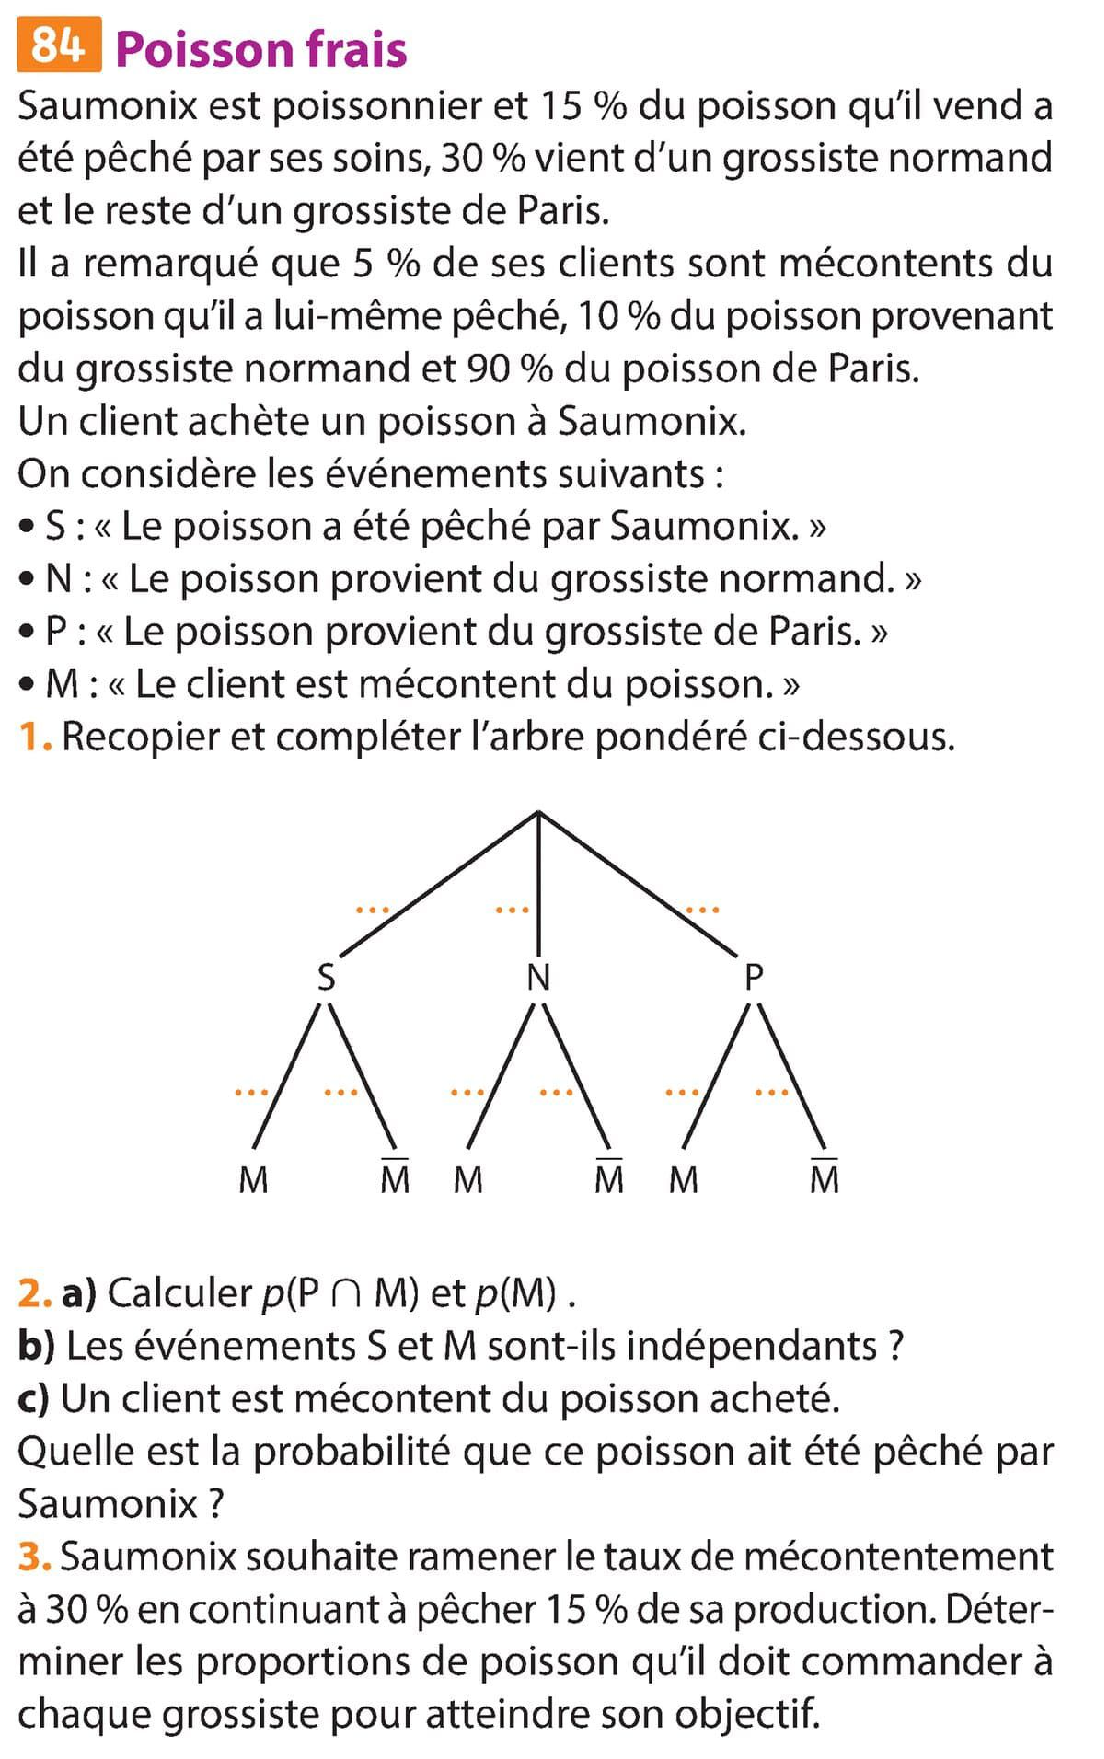
\includegraphics[width=7cm,height=11cm]{Sesamath1ere_84p291.pdf}
			\caption{84 page 291 Sesamath 1ere Spe}
			\label{fig:sesamath1ere84p291}
		\end{figure}		
	
\end{document}